\chapter{Methodology}
\label{ch:intro}

This chapter outlines the methodological foundation of the proposed localization system. It describes the main system components and how they are integrated to estimate the robot’s pose by combining LiDAR and inertial measurements with a pre-built 3D map. The focus is on the overall process and key implementation choices that support accurate and real-time localization.

\section{System Overview}


The proposed localization system estimates the 6-DoF pose of a mobile robot by combining LiDAR and inertial sensor data with a prior 3D map of the environment. The system is designed to operate in real time and deliver accurate, drift-resilient localization in complex, large-scale, and partially dynamic environments.

The localization pipeline begins with preprocessing of the raw LiDAR point cloud. This includes filtering, downsampling, and transformation to a consistent reference frame. To improve robustness in semi-dynamic scenes, transient objects such as vehicles and pedestrians are detected using a deep learning-based 3D object detection model and removed from the scan prior to registration.

In parallel, inertial measurements from the IMU are fused with deskewed LiDAR data using the FAST-LIO2 framework~\cite{xuFastLIO2}, which provides high-frequency odometry estimates through tightly coupled LiDAR-inertial integration. This module ensures locally consistent motion tracking with minimal latency.

To correct drift and maintain alignment with a global reference, the system performs scan-to-map matching. A local submap is dynamically loaded from the global map based on the robot’s current estimated position. Only relevant tiles within a specified radius are retrieved, optimizing memory and computation. The filtered LiDAR scan is then aligned with this submap using a multithreaded Normal Distributions Transform (NDT-OMP) algorithm~\cite{koide2019portable}, which produces a globally referenced pose estimate.

Both odometry and scan-matching results are fused using a fixed-lag smoothing approach based on factor graph optimization. This module maintains a sliding window of recent trajectory states and performs real-time optimization to output a drift-resilient and globally consistent pose estimate.

The overall system architecture and step-by-step algorithm flow are illustrated in Figure~\ref{fig:diagram-map-basedlocalization} and Algorithm~\ref{alg:localization-system}, respectively. The subsequent sections describe each component of the system in detail, including LiDAR preprocessing, local submap loading, odometry estimation, scan matching, graph-based fusion, and dynamic object removal.


%The architecture overview and the complete step-by-step algorithm flow of the proposed localization system are shown in Figure \ref{fig:diagram-map-basedlocalization} and Algorithm \ref{alg:localization-system}. 

%The input of the system includes the raw online point-cloud, raw IMU data as well as the prior map , and output real-time accurate 6 DOF pose.\\	
%The system can be divided in to the following different modules:
%\begin{enumerate}
%	\item Scan Pre-Processing: Performs a series of point cloud processing steps to filter and extract relevant features from the raw LiDAR data.
%	
%	\item LIDAR-INERTIA Odometry - Estimates high-frequency odometry by fusing raw IMU data and LiDAR scans using FAST-LIO\cite{xuFastLIO2} framework. The resulting odometry is added as a local constraint (odom factor) to the factor graph.
%	
%	\item Dynamic Local Map Loading: Generates a local map around the robot’s current pose within a specified radius from the prior map.
%	
%	\item Scan-to-Map Matching: Aligns the current LiDAR scan with the local map to estimate the robot's pose in the prior map using parallelize NDT. The estimated pose is added as a prior constraint (map factor) to the factor graph.
%	
%	\item Sliding Window Factor Graph Optimizer:Fuses odometry and map constraints within a sliding window to optimize and output a real-time, accurate 6-DoF pose.
%	
%	
%\end{enumerate}

\begin{figure}
    \centering
    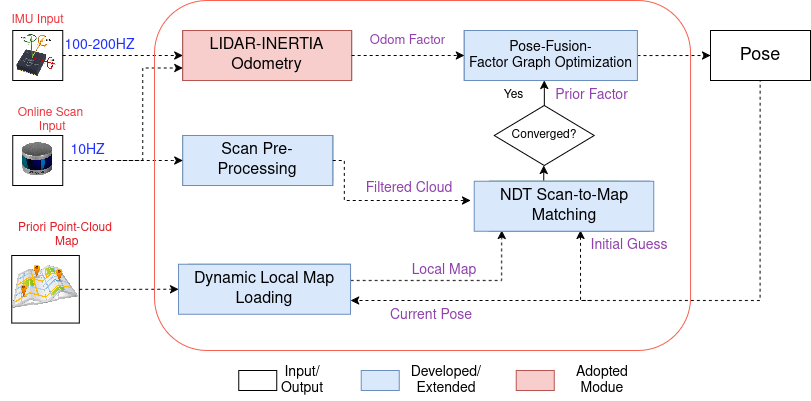
\includegraphics[width=1\linewidth]{images/system-overview.png}
    \caption{Complete Diagram of Map Based Localization}
    \label{fig:diagram-map-basedlocalization}
\end{figure}


\begin{algorithm}[H]
	\caption{LiDAR-Inertial Localization with Prior Map}
	\label{alg:localization-system}
	
	\textbf{Input:} $\mathcal{P}_t$ (LiDAR Point Cloud), $\mathcal{I}_t$ (IMU Data), $\mathcal{M}$ (Prior Map)\\
	\textbf{Output:} $\mathbf{T}_t$ (Real-time 6-DoF Pose)
	
	\begin{algorithmic}[1]
		
		\While{System is running}
		
		\State Acquire LiDAR point cloud $\mathcal{P}_t$ and IMU data $\mathcal{I}_t$
		
		\State Perform scan pre-processing on $\mathcal{P}_t$ to obtain filtered point cloud $\mathcal{P}_t^{filtered}$
		
		\State Estimate LiDAR-Inertial Odometry using $\{\mathcal{P}_t^{filtered}, \mathcal{I}_t\}$ to obtain odometry pose $\mathbf{T}_t^{lio}$	
		
		\If{$|| \mathbf{T}_t - \mathbf{T}_{last}^{map} || > d_{threshold}$}
		\State Load dynamic local map $\mathcal{M}_t^{local}$ from $\mathcal{M}$ centered at $\mathbf{T}_t$
		\State Update $\mathbf{T}_{last}^{map} \gets \mathbf{T}_t$
		\EndIf
		
		\State Perform scan-to-map matching between $\mathcal{P}_t^{filtered}$ and $\mathcal{M}_t^{local}$ to obtain map-based pose $\mathbf{T}_t^{map}$
		
		\If{Matching score $> s_{threshold}$}
		\State Add prior factor with $\mathbf{T}_t^{map}$ to factor graph
		\EndIf
		
		\State Add odometry factor with $\mathbf{T}_t^{lio}$ to factor graph
		
		\State Optimize sliding window factor graph to obtain final pose $\mathbf{T}_t$
		
		\EndWhile
		
	\end{algorithmic}
\end{algorithm}



\subsection{LiDAR Scan Pre-Processing}

Raw LiDAR scans typically produce large point-clouds that vary in density across the range of the sensor. While points near the sensor are densely sampled, those at longer distances become increasingly sparse due to fixed angular resolution. This non-uniform density, combined with measurement noise and dynamic objects, introduces challenges for efficient and robust localization. To address these issues, I apply a structured pre-processing pipeline that filters, reduces, and cleans the incoming data prior to further processing.

As illustrated in Figure~\ref{fig:lidar-preprocessing}, the following steps are applied to each incoming point cloud:

\begin{itemize}
	\item \textbf{Crop-Box Filtering:} I use a spatial crop-box filter to remove points outside a user-defined region of interest centered around the sensor. This step eliminates distant or irrelevant points, reducing computational load and focusing on the region critical for accurate scan alignment.
	
	\item \textbf{Statistical Outlier Removal:} To mitigate the effect of random noise, I apply a statistical filter that removes isolated or spurious measurements. For each point, the average distance to its $k$ nearest neighbors is computed. Points exceeding the global mean by a threshold multiple of the standard deviation are discarded as outliers.
	
	\item \textbf{Voxel-Grid Downsampling:} To reduce data size while preserving geometric structure, I downsample the filtered point cloud using a voxel-grid filter. The space is partitioned into uniform voxels, and all points within each voxel are replaced by their centroid. This ensures that the point cloud remains computationally tractable without compromising registration fidelity.
	
 \item \textbf{Dynamic Object Removal:} To improve robustness in dynamic environments, points associated with moving objects are removed. I use a learning-based detector (CenterPoint) to identify dynamic agents and remove their corresponding points using 3D bounding boxes. Further details are provided in Section~\ref{sec:dynamic_object_removal}.
\end{itemize}

This cleaned and downsampled point-cloud is then used as input to the scan-to-map matching module, where it is aligned with a local submap to estimate the robot's global pose.


\begin{figure}[ht]
	\centering
	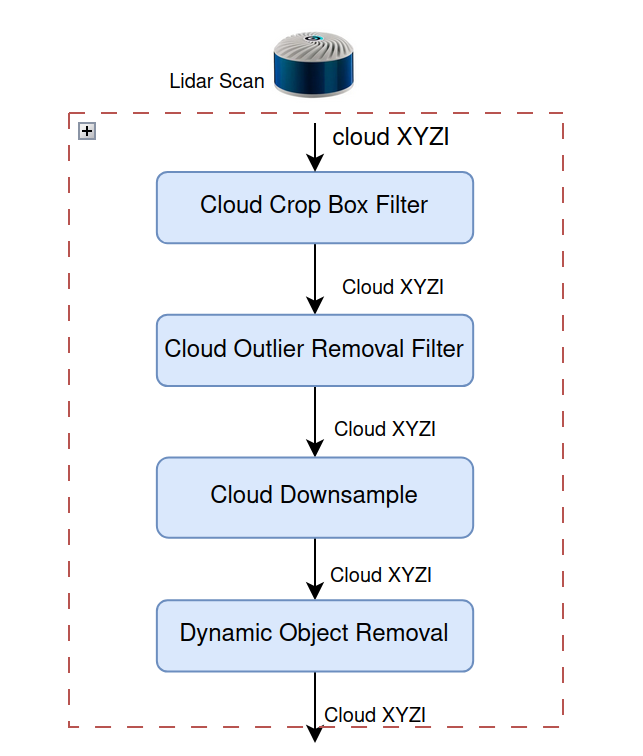
\includegraphics[width=0.4\textwidth]{preproccessing_cloud.png}
\caption{Overview of LiDAR scan pre-processing steps. The raw point cloud undergoes spatial cropping, statistical outlier removal, voxel-grid downsampling, and dynamic object removal.}
\label{fig:lidar-preprocessing}

\end{figure}


%\begin{table}[htbp]
%\centering
%\caption{LiDAR Scan Processing Methods and Parametrs  Across Different Sensor Setups}
%\label{tab:lidar_preprocessing}
%\begin{tabular}{|p{3.5cm}|p{3.5cm}|p{3.5cm}|p{3.5cm}|}
%\hline
%\textbf{Processing Step} & \textbf{KITTI(Velodyne HDL-64E)} & \textbf{MulRan(Ouster-OS1-64)} & \textbf{(Ouster-OS1-128)} \\
%\hline
%LiDAR Type & Velodyne HDL-64E & Ouster OS1-64 & Ouster OS1-128 \\
%% \hline
%% \textbf{Vertical Channels} & 64 & 64 & 128 \\
%% \hline
%% \textbf{Vertical FOV} & $\pm$2° to $\pm$24.8° ($\sim$26.8° total) & $\pm$16.6° ($\sim$33.2° total) & $\pm$22.5° ($\sim$45° total) \\
%\hline
%Max Range & $\sim$120 m & $\sim$120 m & $\sim$240 m \\
%\hline
%Crop Box Filter & 90-100m & 90-100m & 180-200m\\
%\hline
%Downsampling Method & Voxel-Grid(leaf-size: 0.5m) & Voxel-Grid(leaf-size: 0.4-0.6 m) & Voxel-Voxel(0.5-0.8 m) \\
%\hline
%Outlier Removal & Statistical (K=50, Std=1.0) & Statistical (K=40, Std=1.0) & Statistical(K=40 ,Std=1,0) \\
%\hline
%% \textbf{Ground Removal} & Not used & Yes — flat surface segmentation &  Yes — flat surface segmentation \\
%% \hline
%\end{tabular}
%\end{table}

\subsection{Map Pre-Processing}

To support real-time localization in large-scale environments, the global point-cloud map is pre-processed into a 2D grid of tiles each stored as an individual point-cloud file. During this offline division, every point’s \(x\)–\(y\) coordinates are used to assign it to a grid cell of side length \(s\), where \(s\) is chosen to balance tile granularity against file count.Each
grid cell is saved as an individual point cloud file, and its index is stored as metadata for fast
retrieval. During localization, these indexes enable loading only the relevant grids within the
robot’s local map radius, reducing memory usage and improving processing efficiency.

At runtime, I maintain a dynamic local sub-map around the robot by loading only those tiles whose centers lie within a radius
\begin{equation}
	\label{eq:rmap}
	r_{\mathrm{map}} = r_{\mathrm{lidar}} + r_{\mathrm{margin}},
\end{equation}
where \(r_{\mathrm{lidar}}\) is the LiDAR’s maximum range and \(r_{\mathrm{margin}}\) is a small buffer to ensure sufficient overlap for robust scan-to-map matching. To avoid unnecessary I/O, I trigger a map update only when the robot’s current position \(\mathbf{T}_t\) moves farther than a threshold \(d_{\mathrm{thresh}}\) from the last update location \(\mathbf{T}_{\mathrm{last}}\), that is,
\begin{equation}
	\label{eq:load_condition}
	\|\mathbf{T}_t - \mathbf{T}_{\mathrm{last}}\|_2 > d_{\mathrm{thresh}}.
\end{equation}

When equation~\ref{eq:load_condition} is satisfied, the system identifies all grid cells whose centers fall within the circle of radius \(r_{\mathrm{map}}\) about \(\mathbf{T}_t\). Those tiles not yet in memory are loaded from the global map, while any previously loaded tiles that now lie outside this radius are evicted. Finally, \(\mathbf{T}_{\mathrm{last}}\) is updated to the new robot position. This selective, radius-based loading and unloading scheme keeps the local map size bounded, minimizes memory usage, and ensures that scan-to-map matching always operates on the most relevant portion of the prior map.

\section{LIDAR Inertia Odometry} 
FAST-LIO2 serves as the high-frequency LiDAR–Inertial Odometry front-end in our localization pipeline. At each timestep \(t\), the filter ingests IMU angular rate \(\omega_m(t)\) and linear acceleration \(a_m(t)\) (200\,Hz) together with motion-compensated LiDAR point clouds (10\,Hz), deskewed using the same IMU measurements. All sensor data are transformed into a common body frame via the known extrinsic calibration 
\begin{equation}
	T_{\mathrm{imu}\to\mathrm{lidar}}
	\;\in\;SE(3).
\end{equation}
FAST-LIO2 implements a tightly-coupled iterated Kalman filter, directly associating each incoming LiDAR point with the local map using an incremental k-d tree (ikd-Tree), thereby eliminating explicit feature extraction and frame-to-frame scan matching. At each LiDAR update, the filter propagates the state estimate \(\mathbf{x}(t)\) via the IMU pre-integration equations, then corrects it using the residuals between measured points and their expected positions in the map. The result is a 6-DOF pose estimate
\begin{equation}
	\hat{\mathbf{T}}_{WB}(t)
	\;=\;
	\begin{bmatrix}
		\mathbf{R}_{WB}(t) & \mathbf{t}_{WB}(t) \\
		\mathbf{0}           & 1
	\end{bmatrix}
	\;\in\;SE(3),
\end{equation}
which we publish as an odometry factor in our global factor graph. IMU noise densities and bias random-walk coefficients (\(\sigma_\omega, \sigma_a, \sigma_{b_\omega}, \sigma_{b_a}\)) are set according to the manufacturer’s specifications. While FAST-LIO2 exhibits negligible drift over short intervals, residual error on long trajectories is corrected through map matching constraints in the subsequent optimization (Section~\ref{sec:fusion}).


\section{Scan-to-Map Matching}
The Scan-to-Map Matching module is a critical component of the proposed localization system. Its primary objective is to align the current LiDAR scan with a dynamically loaded local submap and estimate the robot’s pose relative to the prior map coordinate frame.Several registration techniques were considered during system design. While Iterative Closest Point (ICP)\cite{BeslICP1992} and the standard Normal Distributions Transform (NDT)\cite{biber2003ndt} are commonly used, they were not selected due to their high computational cost and sensitivity to initial pose estimates.

To overcome these limitations, this work adopts a multithreaded implementation of the Normal Distributions Transform (NDT-OMP)~\cite{koide2019portable}, which leverages OpenMP-based parallelization to significantly accelerate computation. NDT-OMP maintains the robustness of NDT while enabling real-time performance through parallel evaluation of gradients and Hessians during scan registration. This makes it particularly well-suited for large-scale and time-constrained localization tasks.

%
%The Scan-to-Map Matching module is a crucial component of the proposed localization system. Its primary objective is to align the current LiDAR scan with the dynamically loaded local map and estimate the robot's accurate pose within the prior map coordinate frame.In this work, the Normal Distributions Transform (NDT)\cite{biber2003ndt} algorithm is employed for robust and efficient scan registration. Specifically, a multi-threaded implementation of NDT (NDT-OMP) \cite{koide2019portable} is utilized, leveraging OpenMP-based parallelization to accelerate computation and enable real-time performance. 



The module begins by voxelizing the local map: each occupied cell \(i\) is represented by a Gaussian distribution \(\mathcal{N}(\mu_i,\Sigma_i)\) at a resolution \(r\) that balances map fidelity against computational load. Given an initial pose estimate \(\mathbf{p}_0 = [x_0,y_0,z_0,\phi_0,\theta_0,\psi_0]^T\) (from the previous fused pose), the algorithm refines this estimate by minimizing the negative log-likelihood of the transformed scan points under their enclosing Gaussians (more detail Section~\ref{sec:Normal Distributions Transform}):
\[
J(\mathbf{p}) = -\sum_{k=1}^N \log\bigl[\mathcal{N}\bigl(T(\mathbf{p},\mathbf{x}_k)\mid\mu_{c(k)},\Sigma_{c(k)}\bigr)\bigr].
\]


To meet real-time constrain, the computation of gradient(first derivative) and Hessian(second derivative) of the cost function are parallelized over T threads at each Newton iteration (up to \(N_{\max}\)).The set of LIDAR scan points \(\{\mathbf{x}_k\}_{k=1}^N\) partitioned into disjoint subsets \(\{\mathcal{K}_t\}_{t=1}^T\). Each thread \(t\) independently accumulates local gradient and Hessian contributions:

\begin{align}
	\label{eq:local-gradient}
	\mathbf{g}^{(t)}
	&= \sum_{k\in\mathcal{K}_t} \nabla_{\!p}\bigl[-\log p(T(\mathbf{p},\mathbf{x}_k))\bigr],\\
	\label{eq:local-hessian}
	\mathbf{H}^{(t)}
	&= \sum_{k\in\mathcal{K}_t} \nabla^2_{\!p}\bigl[-\log p(T(\mathbf{p},\mathbf{x}_k))\bigr].
\end{align}

After all threads complete, a final reduction merges these into the global quantities.This lock-free design uses per-thread buffers and OpenMP’s guided scheduling to balance uneven voxel densities.


\begin{equation}
	\label{eq:reduction}
	\mathbf{g} = \sum_{t=1}^T \mathbf{g}^{(t)},
	\quad
	\mathbf{H} = \sum_{t=1}^T \mathbf{H}^{(t)}.
\end{equation}


At each iteration the pose update uses a line-search–scaled Newton step:

\begin{equation}
	\label{eq:update}
	\mathbf{p} \;\leftarrow\; \mathbf{p} \;-\; \alpha \,\mathbf{H}(\mathbf{p})^{-1}\,\mathbf{g}(\mathbf{p}),
	\quad
	\alpha \;\in\; [0,1], 
	\quad
	\|\Delta\mathbf{p}\|<\varepsilon.
\end{equation}
The key parameters governing the NDT-OMP scan matching process are summarized in Table~\ref{tab:ndt-omp-params}. These parameters control the resolution of the voxel grid, convergence criteria, optimization behavior, and parallelization strategy.

\begin{table}[ht]
	\centering
	\renewcommand{\arraystretch}{1.1}
	\setlength{\tabcolsep}{6pt}
	\caption{Key parameters of the NDT-OMP Scan-to-Map Matching implementation}
	\label{tab:ndt-omp-params}
	\begin{tabular}{@{}lll@{}}
		\toprule
		\textbf{Parameter}         & \textbf{Symbol}       & \textbf{Description} \\ 
		\midrule
		Voxel resolution           & \(r\)                 & Side length of each map voxel \\ 
		Initial step size          & \(\alpha_0\)          & Starting multiplier for Newton update \\ 
		Convergence threshold      & \(\varepsilon\)       & Minimum norm of pose update for convergence \\ 
		Maximum iterations         & \(N_{\max}\)          & Upper limit on Newton-method iterations \\ 
		Thread count               & \(T\)                 & Number of parallel threads used in optimization \\ 
		\bottomrule
	\end{tabular}
\end{table}

Once scan matching converges, the resulting optimized pose is used as a global correction in the fusion stage, where it is integrated with LiDAR-inertial odometry using a factor graph-based optimization framework.




\section{ Real-Time Factor Graph Optimization }
\label{sec:fusion}

To fuse odometry from FAST-LIO2 with global corrections from scan-to-map matching, a factor graph with fixed-lag smoothing is employed. An Extended Kalman Filter (EKF) was initially considered, using FAST-LIO2 as the prediction model and map-based updates. However, the high-dimensional state of FAST-LIO2, which includes LiDAR–IMU calibration and bias terms, made EKF integration unstable and impractical.

The factor graph approach offers a more modular and scalable solution by modeling each constraint independently and optimizing them jointly. The use of a sliding window limits computation to recent states, ensuring real-time performance.

The following section details the formulation of the factor graph and the types of factors used.

\subsection{Factor Graph Formulation}

We denote the robot trajectory as a sequence of poses:
\begin{equation}
	\mathcal{X} = { \mathbf{x}_0, \mathbf{x}_1, \dots, \mathbf{x}_k }, \quad \mathbf{x}_i \in SE(3)
\end{equation}
where each pose $\mathbf{x}i $  represents the 6-DOF position and orientation of the robot at discrete time step \textit{i} , and SE(3) denotes the special Euclidean group representing 3D rigid body transformations.

\paragraph{1. Prior Factor}
A prior factor is used to anchor the initial pose to a known global reference frame. It models the prior distribution over the initial state , expressed as:
\begin{equation}
	\phi_{\text{prior}}(\mathbf{x}_0) = \exp\left( -\frac{1}{2} | \mathbf{x}_0 - \bar{\mathbf{x}}_0 |^2{\Sigma_0} \right)
\end{equation}

In this formulation, $\mathbf{x}_0$ is the estimated initial pose of the robot. The term $\bar{\mathbf{x}}_0$ denotes the prior mean pose from the first LIO output or initialization, and $\mathbf{{\Sigma_0}}$ is the prior covariance matrix reflecting the uncertainty. This Gaussian prior serves as a fixed anchor to stabilize the trajectory estimation.

\paragraph{2. Odometry (Between) Factors}
Relative motion from LIO is encoded using between factors, which represent the relative transformation between consecutive poses:
\begin{equation}
	\phi_{\text{odom}}(\mathbf{x}{i-1}, \mathbf{x}i) = \exp\left( -\frac{1}{2} \left| f{\text{odom}}(\mathbf{x}_{i-1}, \mathbf{x}i) - \bar{\mathbf{z}}i^{\text{odom}} \right|^2{\Sigma{\text{odom}}} \right)
\end{equation}
Here,$\bar{\mathbf{z}}i^{\text{odom}}$ is the relative pose measurement between time steps $\text{\textit{i}}$  and $\text{\textit{i+1}}$, derived from the LIO module. The $f{\text{odom}(\mathbf{.})}$
function  calculates the predicted relative transformation between the estimated poses $\mathbf{x}_{i-1}$ and $\mathbf{x}_{i},$ . The $ \mathbf{\Sigma{\text{odom}}}$ term   is the associated covariance matrix, which quantifies the uncertainty in the odometry measurement. These between factors form the sequential backbone of the trajectory by chaining consecutive pose estimates together through relative motion constraints.

\paragraph{3. Map-Matching Priors}
Absolute pose estimates derived from scan-to-map matching using Normal Distributions Transform (NDT) are incorporated as prior constraints on select poses:
\begin{equation}
	\phi_{\text{map}}(\mathbf{x}_j) = \exp\left( -\frac{1}{2} | \mathbf{x}j - \bar{\mathbf{x}}j^{\text{map}} |^2{\Sigma{\text{map}}} \right)
\end{equation}
In this expression, $\bar{\mathbf{x}}j^{\text{map}} $  denotes the global pose obtained by aligning the current LiDAR scan with a pre-built prior map using scan matching techniques. The associated covariance matrix $\mathbf{\Sigma{\text{map}}}$ expresses the uncertainty of the registration process, accounting for alignment quality and sensor noise. These priors provide absolute spatial constraints within the factor graph, which help to correct accumulated drift from relative odometry and enhance the global consistency of the trajectory estimation.
\subsection{Maximum A Posteriori (MAP) Estimation}

The objective of the sensor fusion system is to compute the most probable robot trajectory given all available measurements, including odometry and map-matching observations. This is formulated as a Maximum A Posteriori (MAP) estimation problem, expressed as the following nonlinear least-squares objective:

\begin{equation}
	\mathbf{X}^* = \arg\min_{\mathbf{X}} \left(
	\| \mathbf{x}_0 - \bar{\mathbf{x}}_0 \|^2_{\Sigma_0} +
	\sum_{i=1}^{k} \left\| f_{\text{odom}}(\mathbf{x}_{i-1}, \mathbf{x}_i) - \bar{\mathbf{z}}_i^{\text{odom}} \right\|^2_{\Sigma_{\text{odom}}} +
	\sum_{j \in \mathcal{M}} \left\| \mathbf{x}_j - \bar{\mathbf{x}}_j^{\text{map}} \right\|^2_{\Sigma_{\text{map}}}
	\right)
	\label{eq:map-estimation}
\end{equation}

\begin{comment}
	Here:
	\begin{itemize}
		\item \( \mathbf{X} = \{ \mathbf{x}_0, \mathbf{x}_1, \dots, \mathbf{x}_k \} \) is the sequence of robot poses to be estimated.
		\item \( \bar{\mathbf{x}}_0 \) is the prior estimate of the initial pose, with covariance \( \Sigma_0 \).
		\item \( \bar{\mathbf{z}}_i^{\text{odom}} \) is the observed relative transformation between \( \mathbf{x}_{i-1} \) and \( \mathbf{x}_i \) from LiDAR-inertial odometry, with associated covariance \( \Sigma_{\text{odom}} \).
		\item \( f_{\text{odom}}(\cdot) \) is the motion model predicting the relative transformation between consecutive poses.
		\item \( \bar{\mathbf{x}}_j^{\text{map}} \) represents the pose obtained from map-matching at selected indices \( j \in \mathcal{M} \), with uncertainty \( \Sigma_{\text{map}} \).
	\end{itemize}
\end{comment}

Each term in the cost function represents a Mahalanobis distance, penalizing deviations from the respective measurements weighted by their uncertainty. Solving this objective yields the optimal trajectory estimate \( \mathbf{X}^* \), which fuses relative odometry and global pose observations in a probabilistically consistent manner.


\subsection{Fixed-Lag Smoothing and Marginalization}

In our proposed system, fixed-lag smoothing is used to maintain real-time performance while optimizing the recent trajectory of the robot. Instead of keeping the entire history of poses in the factor graph, we define a sliding time window of length \( \tau \), such that only poses within the interval \( [t_k - \tau, t_k] \) are retained, where \( t_k \) is the current time. This ensures that the graph grows only within a fixed temporal horizon, regardless of how long the system has been running.

Let \( \mathbf{x}_0, \mathbf{x}_1, \dots, \mathbf{x}_k \) represent the sequence of robot poses over time. At each time step, the latest pose \( \mathbf{x}_k \) is added to the factor graph along with new factors derived from LIO (odometry) and map-matching. Older poses such as \( \mathbf{x}_i \) for which \( t_i < t_k - \tau \) are marginalized out to limit the graph size.

The process of marginalization involves removing a variable (pose) from the graph while preserving its influence on the remaining variables. Suppose the state vector is partitioned as:
\begin{equation}
	\mathbf{x} = \begin{bmatrix} \mathbf{x}_m \\ \mathbf{x}_r \end{bmatrix},
\end{equation}
where \( \mathbf{x}_m \) are the variables to be marginalized (e.g., old poses outside the lag window), and \( \mathbf{x}_r \) are the variables retained in the active window. The joint probability distribution is expressed as:
\begin{equation}
	P(\mathbf{x}_m, \mathbf{x}_r) = P(\mathbf{x}_m | \mathbf{x}_r) P(\mathbf{x}_r).
\end{equation}
To obtain a reduced representation, we marginalize out \( \mathbf{x}_m \):
\begin{equation}
	P(\mathbf{x}_r) = \int P(\mathbf{x}_m, \mathbf{x}_r) \, d\mathbf{x}_m.
\end{equation}

As a result, a new dense factor is introduced between variables in \( \mathbf{x}_r \) that were connected to \( \mathbf{x}_m \), preserving the influence of the eliminated variables.

\begin{figure}[htbp]
	\centering
	\begin{subfigure}[b]{0.5\textwidth}
		\centering
		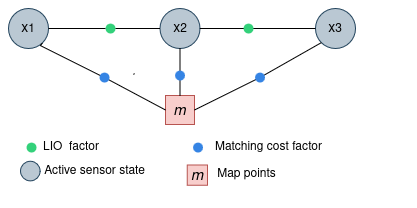
\includegraphics[width=\textwidth]{images/fixed_lag_smooth_a.png}
		 \captionsetup{width=2\textwidth}
		\caption{The initial factor graph contains active states \( \mathbf{x}_1 \) to \( \mathbf{x}_3 \), linked through LiDAR-inertial odometry (LIO) and map-matching factors. }
		\label{fig:bayes-a}
	\end{subfigure}
		\vskip\baselineskip
	\begin{subfigure}[b]{0.5\textwidth}
		\centering
		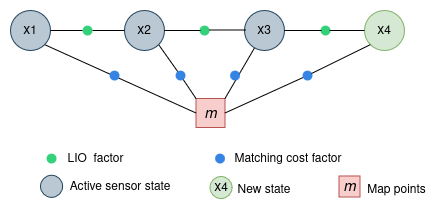
\includegraphics[width=\textwidth]{images/fixed_lag_smooth_b.png}
		\captionsetup{width=2\textwidth}
		\caption{A new state \( \mathbf{x}_4 \) is introduced, remaining within the lag window. }
		\label{fig:bayes-b}
	\end{subfigure}
	\vskip\baselineskip
	\begin{subfigure}[b]{0.7\textwidth}
		\centering
		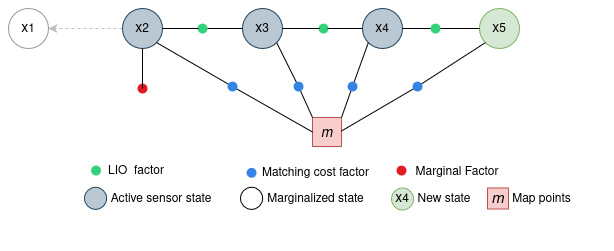
\includegraphics[width=\textwidth]{images/fixed_lag_smooth_c.png}
		\captionsetup{width=1.2\textwidth}
		
		\caption{As state \( \mathbf{x}_5 \) is added, the oldest state \( \mathbf{x}_1 \) is marginalized and its influence is preserved via a prior factor. 
		}
		\label{fig:bayes-c}
	\end{subfigure}
    \vskip\baselineskip
	\begin{subfigure}[b]{0.7\textwidth}
		\centering
		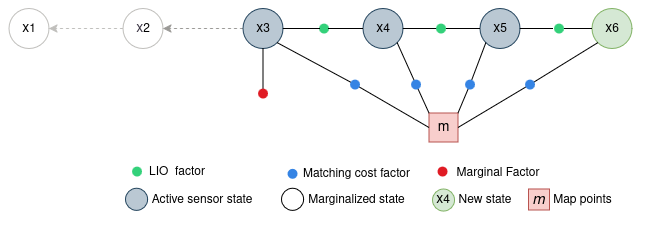
\includegraphics[width=\textwidth]{images/fixed_lag_smooth_d.png}
		\captionsetup{width=1.2\textwidth}
		\caption{At time \( t_6 \), \( \mathbf{x}_6 \) is introduced and \( \mathbf{x}_2 \) is marginalized, maintaining a fixed-lag window over the most recent four states. 
	}
		\label{fig:bayes-d}
	\end{subfigure}
    \vskip\baselineskip
	\caption{Demonstration of fixed-lag smoothing with a lag size of \( n = 4 \) in a factor graph-based localization system.}
	\label{fig:fixed-lag-example}
\end{figure}

The process of fixed-lag smoothing is illustrated in Figure~\ref{fig:fixed-lag-example} using a temporal window of length \( n = 4 \). Initially (Figure~\ref{fig:bayes-a}), the system contains states \( \mathbf{x}_1 \), \( \mathbf{x}_2 \), and \( \mathbf{x}_3 \), connected by odometry and map-matching factors. As pose \( \mathbf{x}_4 \) is added at time \( t_4 \) (Figure~\ref{fig:bayes-b}), it links to \( \mathbf{x}_3 \) through a new odometry factor and includes a map constraint. Since all poses \( \mathbf{x}_1 \) to \( \mathbf{x}_4 \) lie within the lag window \( [t_1, t_4] \), the graph remains fully active and no marginalization occurs.


When the system reaches time step \( t_5 \), pose \( \mathbf{x}_5 \) is added, along with its corresponding odometry and map-matching constraints. At this point, pose \( \mathbf{x}_1 \) falls outside the fixed-lag window \( [t_2, t_5] \). As a result, it is marginalized. This process eliminates \( \mathbf{x}_1 \) from the graph but replaces its influence with a dense prior that connects to the remaining relevant states, particularly \( \mathbf{x}_2 \) and beyond (Figure~\ref{fig:bayes-c}). The marginalized node is no longer directly optimized, but its effect is preserved through conditional probability in the form of a Bayes net.

At the next step, time \( t_6 \), a new pose \( \mathbf{x}_6 \) is introduced. To maintain the lag window \( [t_3, t_6] \), the system marginalizes pose \( \mathbf{x}_2 \), introducing another dense factor that connects to the active variables. The current active states now consist of \( \mathbf{x}_3 \), \( \mathbf{x}_4 \), \( \mathbf{x}_5 \), and \( \mathbf{x}_6 \), all within the sliding lag window (Figure~\ref{fig:bayes-d}).

This incremental update mechanism, implemented using the GTSAM library, maintains a bounded graph size by marginalizing old variables into Bayes net conditionals while preserving historical information. Recent poses within the active window are kept in a factor graph and updated via iSAM2, striking a balance between computational efficiency and estimation accuracy for real-time localization.

\subsection{Outlier Rejection via Mahalanobis Distance}

To ensure robust fusion of odometry and scan–map correction constraints, we apply a probabilistic outlier test based on the Mahalanobis distance. Let the correction measurement be the 6-DOF pose  
\(\mathbf{z} = [x, y, z, \phi, \theta, \psi]^\mathsf{T}\)  
provided by the NDT-based scan matching, with associated covariance \(\mathbf{\Sigma}_z\). Given the current filter estimate \(\hat{\mathbf{z}}\), we compute the innovation  
\[
\Delta \mathbf{z} \;=\; \mathbf{z} - \hat{\mathbf{z}}.
\]  
The squared Mahalanobis distance is then
\begin{equation}
	\label{eq:mahalanobis}
	D_M^2 \;=\;\Delta \mathbf{z}^\mathsf{T}\,\mathbf{\Sigma}_z^{-1}\,\Delta \mathbf{z}.
\end{equation}
Under the Gaussian assumption, \(D_M^2\) follows a \(\chi^2\) distribution with \(d=6\) degrees of freedom. We reject the correction if
\begin{equation}
	\label{eq:threshold}
	D_M^2 \;>\;\chi^2_{d,\,0.95},
\end{equation}
where \(\chi^2_{d,\,0.95}\) is the 95\% quantile of the \(\chi^2_d\) distribution. Otherwise, the measurement is accepted and incorporated into the factor graph. This criterion effectively discards implausible scan-matching corrections while preserving valid global pose updates.


\section{Dynamic Object Detection and Removal}
\label{sec:dynamic_object_removal}
\subsection{Dynamic Object Detection}

To identify and remove dynamic objects from the LiDAR point cloud, this work utilizes a deep learning-based 3D object detection pipeline based on CenterPoint\cite{yin2021center}. The model is developed and trained using the MMDetection3D framework\cite{mmdet3d2020}, and is deployed for real-time inference using the Autoware-compatible implementation\cite{autoware_universe}.

The detection architecture adopts the two-stage design of CenterPoint, as shown in Figure \ref{fig:Overview-CenterPoint }. First, the raw LiDAR point cloud is voxelized and processed by a voxel feature encoder and a PointPillars-based sparse convolutional backbone\cite{lang2019pointpillars}, which extracts high-level spatial features. These features are projected into a Bird’s-Eye View (BEV) map, enabling efficient object detection. A keypoint-based detection head then identifies object centers and regresses 3D bounding box attributes, including size, orientation, and velocity. The final output includes class-labeled 3D detections, which are used to support dynamic object removal.

Instead of training from scratch, this work utilizes a pretrained CenterPoint model trained on the nuScenes dataset \cite{caesar2020nuscenes}, comprising over 28k LiDAR frames. The model includes five object classes: CAR, TRUCK, BUS, BICYCLE, and PEDESTRIAN. These categories cover the primary dynamic agents present in urban driving scenarios. After training, the model is exported to the ONNX (Open Neural Network Exchange) format, which supports cross-platform deployment and enables hardware-accelerated inference using TensorRT.




\subsection{Detected Object removal }


Following object detection, dynamic elements are removed from the LiDAR point cloud using their predicted 3D bounding boxes. For each detected object, its position, dimensions, and orientation are used to define an oriented 3D cropping volume. These bounding boxes are expanded slightly with a fixed margin to ensure full exclusion of the object’s points, accounting for detection uncertainty or sensor noise.

Each bounding box is then used to define a geometric filter in 3D space. The removal process involves identifying all LiDAR points that fall within the transformed bounding box and excluding them from the original scan. This is performed iteratively for all detected dynamic objects in each frame. The result is a filtered point cloud that retains only static environmental features, which are then used for downstream localization tasks. 


\section{Environmental Noise Simulation}
\label{sec:fog_simulation}

To assess the robustness of the proposed localization pipeline under adverse conditions, we simulate the impact of atmospheric fog on LiDAR scans. Fog causes scattering and absorption of laser beams, leading to partial loss of valid returns, the appearance of false near-field echoes, and a reduction in return intensity. Our simulation adopts the physically grounded model proposed by Teufel et al.~\cite{teufel2022realistic}, applied only to live LiDAR scans. The degradation severity is controlled by the \textit{meteorological visibility} \( V \) (in meters), defined as the maximum distance at which an object can be reliably seen under foggy conditions.

The fog model introduces three major effects, each governed by simple visibility-dependent equations: \textit{(i)} deletion of real points, \textit{(ii)} modification into near-sensor backscatter points, and \textit{(iii)} intensity attenuation.

\subparagraph{Point Deletion.}
Real LiDAR returns are probabilistically removed based on their distance \( d \) and visibility \( V \), using:
\[
p_{\text{delete}}(d) = \frac{a \cdot e^{bV}}{a \cdot e^{bV} + 1}
\]
Here, \( a = -0.70 \) and \( b = -0.024 \) are empirically derived constants that define the effect of fog density on the likelihood of return loss. Deletion probability increases with distance and with denser fog (lower \( V \)).

\subparagraph{Backscatter Modification.}
Points that are not deleted may be converted into \textit{false returns}, simulating backscatter from fog droplets. The probability of modification increases with distance:
\[
p_{\text{modify}}(d) = 1 - e^{-d \cdot \epsilon}, \quad \epsilon = 0.23 \cdot e^{-0.0082V}
\]
The new range is drawn from an exponential distribution:
\[
f(x) = \frac{1}{\lambda} e^{-x / \lambda}, \quad \lambda = -0.006 \cdot V + 2.31
\]
This causes the point to be radially pulled closer to the sensor, mimicking typical fog backscatter effects.

\subparagraph{Intensity Attenuation.}
Return intensity is reduced due to scattering loss along the beam path:
\[
I(d) = I_0 \cdot e^{-\gamma d}, \quad \gamma = 0.02
\]
Points with final intensity below a threshold (e.g., 1000 for 16-bit returns) are discarded. Simulated backscatter points are assigned random intensities in the range of 0--32\% of the maximum value, consistent with real sensor behavior under fog.

\begin{table}[H]
	\centering
	\caption{Fog severity levels based on visibility range}
	\label{tab:noise_levels}
	\begin{tabular}{lc}
		\toprule
		\textbf{Fog Level} & \textbf{Visibility \( V \) (m)} \\
		\midrule
		Mild      & 100 \\
		Moderate  & 60  \\
		Severe    & 30  \\
		\bottomrule
	\end{tabular}
\end{table}

This fog simulation enables a physically interpretable, parameterized degradation model suitable for evaluating localization performance under various visibility conditions.


